\documentclass{article}

\PassOptionsToPackage{numbers,compress}{natbib}
\usepackage{neurips_2026}

\usepackage[utf8]{inputenc}
\usepackage[T1]{fontenc}
\usepackage{hyperref}
\usepackage{url}
\usepackage{booktabs}
\usepackage{amsfonts}
\usepackage{amsmath}
\usepackage{amssymb}
\usepackage{microtype}
\usepackage{xcolor}
\usepackage{graphicx}
\graphicspath{{figures/}}

\title{Routing Visual Evidence Under Domain Shift: Three-Way Factorization for Cross-Domain Audio-Visual Deepfake Detection}

\author{%
  Zhili Nicholas Liang \\
  University of Melbourne \\
  Melbourne, Victoria, Australia \\
  \texttt{nnliang@student.unimelb.edu.au} \\
  \And
  Soyeon Caren Han \\
  University of Melbourne \\
  Melbourne, Victoria, Australia \\
  \texttt{caren.han@unimelb.edu.au} \\
  \And
  Qizhou Wang \\
  University of Melbourne \\
  Melbourne, Victoria, Australia \\
  \texttt{mike.wang@unimelb.edu.au} \\
  \And
  Christopher Leckie \\
  University of Melbourne \\
  Melbourne, Victoria, Australia \\
  \texttt{caleckie@unimelb.edu.au} \\
}

\newcommand{\method}{\textsc{TriRoute}}
\newcommand{\R}{\mathbb{R}}

\begin{document}

\maketitle

\begin{abstract}
Multimodal models are expected to integrate complementary signals across modalities, yet in practice they often rely on spurious shortcuts from a single modality. A common approach to mitigate this issue is to enforce invariance through regularization or domain-adversarial objectives. However, it remains unclear whether such methods actually change how models make decisions, or merely reshape representations without altering their usage.

In this work, we show that improving robustness in multimodal learning is not primarily a problem of enforcing invariance, but of structuring how information is routed. We demonstrate that loss-level interventions, including label-aware domain adversarial training, fail to resolve representation-level entanglement in standard binary decompositions, where modality-specific signals and domain nuisance remain mixed.

We then introduce a simple three-way factorization that separates shared, modality-specific task-relevant, and residual domain-dominant components. This structural change leads to a qualitatively different behavior: performance gains are concentrated on settings that require reliance on the correct modality, and are not observed when applying the same objectives without factorization.

Crucially, we provide multiple lines of evidence that the improvement arises from a change in inference-time routing rather than representation invariance. On the AV1M$\rightarrow$FakeAVCeleb benchmark, \method\ improves the diagnostic FV-RA category from $0.523$ AUC for a two-way baseline to $0.731$ without target data and $0.804$ with unlabelled real-only target clips. Subspace probing shows that the factorized model learns a visual-unique component that is more predictive under distribution shift. Head ablation and progressive masking further reveal that predictions depend critically on this component, whereas non-factorized models remain largely insensitive.

Together, our results suggest a shift in perspective: instead of suppressing spurious signals, multimodal robustness can be achieved by restructuring the pathways through which decisions are made.
\end{abstract}

\section{Introduction}

Multimodal learning aims to combine complementary information from different sources such as vision and audio. In principle, this should enable models to make robust decisions even when one modality is unreliable. In practice, however, multimodal models often collapse to shortcut solutions, relying on the easiest available signal rather than integrating evidence across modalities. This issue becomes particularly evident under modality conflict, where correct predictions require prioritizing one modality over another.

A dominant line of work attempts to address this problem by enforcing invariance, for example through domain adversarial training or regularization. These approaches aim to remove spurious correlations from learned representations, under the assumption that robustness follows from eliminating nuisance information.

However, this assumption remains largely untested. Improvements in out-of-distribution performance are typically interpreted as evidence of better representations, but this does not establish whether models actually use the intended modality at inference time. In particular, existing methods do not distinguish between two fundamentally different possibilities: the model learns a better representation, or the model changes how it routes information when making decisions. This distinction is critical, yet rarely examined directly.

In this work, we show that in standard binary decompositions, loss-level interventions are insufficient to resolve this issue. Even with label-aware domain adversarial objectives, modality-specific task signals and domain-related nuisance remain entangled within the same branch. As a result, the model lacks a structural mechanism to separate useful modality information from spurious signals, and performance gains remain limited. We argue that the problem is therefore not primarily one of objective design, but of representational structure.

To address this, we introduce a simple three-way factorization that decomposes multimodal representations into (1) shared information, (2) modality-specific but task-relevant components, and (3) residual domain-dominant signals.

This decomposition provides an explicit pathway for modality-specific information, removing the need to encode it within a single ``spurious'' branch.

Our empirical results reveal a consistent pattern. First, performance improvements are concentrated in diagnostic settings that require reliance on the correct modality, while other categories remain near ceiling. Second, controlled experiments show that these gains cannot be explained by additional objectives alone, and only emerge when the representation is factorized.

More importantly, we provide direct evidence that the effect is driven by a change in inference-time routing. Subspace probing shows that the modality-specific component learned by the factorized model is more robust under distribution shift. Head ablation and progressive masking further demonstrate that predictions depend critically on this component, whereas non-factorized models remain largely insensitive. Notably, domain information remains present in the representation, indicating that robustness is achieved without enforcing invariance.

These findings suggest a different perspective on multimodal robustness. Rather than attempting to remove spurious signals from representations, it may be more effective to structure representations such that models are encouraged to route decisions through the appropriate modality.

We summarize our contributions as follows:
\begin{itemize}
\item We show that loss-level approaches fail to disentangle modality-specific and domain signals in standard binary decompositions.
\item We introduce a simple three-way factorization that provides a dedicated pathway for modality-specific task-relevant information.
\item We provide multiple lines of evidence that improvements arise from changes in inference-time routing rather than representation invariance.
\item We offer a new perspective on mitigating shortcut learning by focusing on structural routing instead of feature suppression.
\end{itemize}

\section{Related Work}

\paragraph{Audio-visual deepfake detection.}
Multimodal deepfake detection leverages the fact that realistic speech, lip motion, and facial dynamics must stay mutually consistent over time. Early work explored direct audio-visual fusion and synchronization cues \citep{zhou2021jointav, chung2016syncnet}. More recent methods use self-supervised anomaly detection, speech representation learning, or explicit combinations of modality-shared semantic mismatch and modality-specific forensic traces \citep{feng2023avad, liang2024speechforensics, smeu2025avhalign, du2025cad}. These approaches are more robust than purely artifact-based detectors, but most still optimize a single prediction pathway and therefore do not directly test which subspace the detector routes its decisions through under shift.

\paragraph{Evaluation protocols.}
Most audio-visual deepfake work still reports in-dataset or within-benchmark splits. FakeAVCeleb-based evaluation commonly uses train/test splits and leave-one-manipulation protocols \citep{feng2023avad, oorloff2024avff}, while AV-Deepfake1M reports official in-dataset benchmarks on AV1M, LAV-DF, and FAVC \citep{cai2024avdeepfake1m}. The closest prior cross-dataset bridge is AVH-Align, which reports supervised AV1M$\rightarrow$FAVC scores while diagnosing leading-silence shortcuts \citep{smeu2025avhalign}. Our contribution is therefore not the existence of FakeAVCeleb as a target dataset, but an AV1M$\rightarrow$FAVC cross-domain stress test with modality-category reporting and routing analyses focused on FV-RA.

\paragraph{Speech-aware multimodal representations.}
Large-scale audio-visual speech models, such as AV-HuBERT \citep{shi2022avhubert}, learn strong multimodal features that capture both local synchronization and longer-term speech structure. Such representations have proven useful beyond recognition, including forensic analysis and synchronization-based detection \citep{liang2024speechforensics, smeu2025avhalign}. Our method uses the same intuition, but adds an explicit factorization layer so that the downstream detector can discard nuisance factors instead of letting them leak into the prediction head.

\paragraph{Multimodal factorization.}
Generic multimodal representation learning has explored decomposing features into shared/synergistic, unique, and redundant components. The closest such prior is FCD \citep{liu2025fcd}, a plug-and-play factorization for general multimodal prediction that reserves synergistic and unique factors while removing redundant, task-agnostic uncertainty. \method\ uses a related three-part vocabulary, but the residual factor has the opposite operational role. In FCD-style decompositions, the residual or redundant component is primarily unwanted uncertainty to suppress. In \method, the residual is an intentionally supervised \emph{information sink}: it is trained to retain domain-predictive shortcut evidence, is structurally excluded from the fake classifier, and is paired with adversarial pressure only on the task branch. The resulting design is therefore not a generic decomposition module, but a domain-routing mechanism: shortcut evidence is attracted into $Z_{\mathrm{res}}$ while the prediction path is forced to rely on shared content and modality-unique manipulation cues.

This design is related to, but distinct from, earlier shared-private and debiasing lines. Domain Separation Networks (DSN) explicitly split shared and private domain components for adaptation \citep{bousmalis2016dsn}, and DIVA learns separate latent variables for domain, class, and residual variation in a generative framework \citep{ilse2019diva}. Bias-adversarial approaches such as Learning Not to Learn \citep{kim2019learningnottolearn} and Learning from Failure \citep{nam2020learningfromfailure} suppress shortcut exploitation through adversarial or dual-network training. Our method differs in the combination of three properties used together for routing control: (i) a supervised domain-predictive residual sink, (ii) structural exclusion of that sink from the fake head, and (iii) explicit routing validation under cross-domain FV-RA stress tests.

\paragraph{Domain alignment and adversarial adaptation.}
Classical unsupervised domain adaptation often tries to make source and target features globally aligned. DANN \citep{ganin2016dann} trains a gradient-reversal domain classifier on top of the feature representation so that the encoder learns features from which the domain is difficult to predict. CORAL-style alignment instead matches second-order feature statistics across domains, either as a shallow covariance transform or as a differentiable deep loss \citep{sun2016deepcoral}. Both families are useful generic adaptation tools, but in cross-domain audio-visual forensics their pressure can be misdirected when applied to an undifferentiated representation: domain-correlated nuisance, speech content, and manipulation evidence may be entangled, so global alignment can suppress useful forensic signal or leave the final classifier free to route through remaining shortcuts. Our design changes the question from ``can all features be aligned?'' to ``which features is the detector allowed to use?'' We separate a dedicated residual branch whose role is to absorb domain-correlated signal, pair it with a forward domain-prediction objective ($\mathcal{L}_{\mathrm{dom}}$), and apply adversarial pressure only to the task branch. In this sense, \method\ is complementary to DANN/CORAL: it does not merely align all features, but changes the admissible prediction subspace.

\section{Problem Setting}

We study cross-dataset audio-visual deepfake detection. Let $\mathcal{D} = \{(x_i^v, x_i^a, y_i, d_i)\}_{i=1}^N$ denote training samples where $x_i^v$ is a sequence of visual observations, $x_i^a$ is the synchronized audio, $y_i \in \{0,1\}$ is the video-level real/fake label, and $d_i \in \{1,\dots,M\}$ indicates a nuisance partition available during training. Training uses AV-Deepfake1M clips for task supervision. Domain or nuisance supervision is provided in two settings: (i)~a strict \emph{no-target-data} setting using source-side speaker-group pseudo-labels derived from AV1M ($d=0$ or $d=1$ by speaker-ID hash), so no FakeAVCeleb data is used at any stage; and (ii)~a standard \emph{unsupervised domain adaptation} (UDA) setting that additionally uses unlabelled real-only clips from FakeAVCeleb as target domain identity, with no manipulation labels used. In both cases, the target test labels are never observed during training, validation, checkpoint selection, or hyperparameter selection.

Our goal is to learn a scoring function $f(x^v, x^a)$ that remains predictive when the nuisance statistics associated with $d$ shift at test time. We therefore seek a representation in which manipulation evidence remains discriminative for $y$, while predictable but non-transferable signals are isolated rather than implicitly used by the classifier. We do not claim that the learned task branch becomes fully domain-invariant; the claim we test is weaker and more mechanism-focused: factorization changes representation usage and downstream routing under shift.

\section{Method}

\subsection{Overview}

Figure~\ref{fig:overview} gives a conceptual overview of \method. Audio-visual forensics under dataset shift requires separating exactly three qualitatively distinct signal types: cross-modal speech content that should generalize across datasets, modality-unique manipulation evidence that is the detection target, and domain-correlated nuisance that must not reach the prediction head. We therefore design a three-branch factorization in which each branch has an explicit semantic role and a corresponding supervision signal, and the prediction head is structurally restricted to the first two. Starting from frozen AV-HuBERT features $z_v, z_a \in \R^{1024}$, we first extract shared cross-modal factors and modality-specific hidden states:
\begin{equation}
\big[s_v, h_v\big] = F_v(z_v), \qquad \big[s_a, h_a\big] = F_a(z_a),
\end{equation}
where $s_v$ and $s_a$ denote shared task-relevant factors and $h_v, h_a$ collect the remaining modality-specific signal. We then split the modality-specific states into unique task-relevant and residual components:

\begin{equation}
\big[u_v, r_v\big] = G_v(h_v), \qquad \big[u_a, r_a\big] = G_a(h_a).
\end{equation}
Here $u_v$ and $u_a$ are modality-unique task factors, while $r_v$ and $r_a$ form the residual branch that is allowed to absorb shortcut and domain signal. The task representation and residual representation are
\begin{equation}
Z_{\mathrm{task}} = \mathrm{cat}(s_v, u_v, s_a, u_a), \qquad
Z_{\mathrm{res}} = \mathrm{cat}(r_v, r_a).
\end{equation}
For readability, we refer to the shared factor as \emph{content}, the visual-unique task factor as the key \emph{manipulation} carrier for FV-RA, and the residual branch as the \emph{domain} factor.

\subsection{Three-Way Factorization}

\paragraph{Manipulation factor.}
The manipulation factor is intended to encode modality-unique evidence that cannot be explained by authentic cross-modal correspondence. In practice, the visual-unique component $u_v$ is the most important carrier for the visual-fake category FV-RA, while $u_a$ supports audio-fake cases. These unique components feed the task head together with the shared factors.

\paragraph{Content factor.}
The content factor captures shared speech semantics and identity-preserving motion that should remain useful across domains. We align the shared factors across modalities using an audio-visual alignment objective:
\begin{equation}
\mathcal{L}_{\mathrm{align}} = - \sum_{t=1}^T
\log
\frac{\exp(\mathrm{sim}(s_{v,t}, s_{a,t})/\tau)}
{\sum_{j \in \mathcal{N}(t)} \exp(\mathrm{sim}(s_{v,t}, s_{a,j})/\tau)},
\end{equation}
where $\mathrm{sim}(\cdot,\cdot)$ is cosine similarity, $\tau$ is a temperature, and $\mathcal{N}(t)$ is a local temporal window.

\paragraph{Domain factor.}
The residual branch is explicitly optimized to predict the source domain:
\begin{equation}
\mathcal{L}_{\mathrm{dom}} = \mathrm{CE}(C_d(Z_{\mathrm{res}}), d).
\end{equation}
This branch acts as an information sink for codec, resolution, acquisition, and dataset-construction artifacts.

\subsection{Detection and Domain Push-Pull Objectives}

We predict a clip-level fake probability from the task representation:
\begin{equation}
\hat{y} = C_y(Z_{\mathrm{task}}),
\end{equation}
and optimize binary cross-entropy:
\begin{equation}
\mathcal{L}_{\mathrm{fake}} = \mathrm{BCE}(\hat{y}, y).
\end{equation}

To keep task-relevant and residual factors separated, we apply an orthogonality penalty between them:
\begin{equation}
\mathcal{L}_{\mathrm{ortho}} =
\left\| s_v^\top r_v \right\|_F^2
+ \left\| s_a^\top r_a \right\|_F^2
+ \left\| u_v^\top r_v \right\|_F^2
+ \left\| u_a^\top r_a \right\|_F^2.
\end{equation}

To suppress easy domain prediction from the task branch, we apply a gradient-reversal domain classifier:
\begin{equation}
\mathcal{L}_{\mathrm{adv}} =
\mathrm{CE}(C_{\mathrm{adv}}(\mathrm{GRL}(Z_{\mathrm{task}})), d),
\end{equation}
while $\mathcal{L}_{\mathrm{dom}}$ simultaneously attracts domain information into $Z_{\mathrm{res}}$. This push-pull effect does not aim to make $Z_{\mathrm{task}}$ fully domain-invariant; instead it makes shortcut routing into the prediction head less attractive.

The full objective is
\begin{equation}
\mathcal{L}
=
\mathcal{L}_{\mathrm{fake}}
+
\lambda_{\mathrm{align}} \mathcal{L}_{\mathrm{align}}
+
\lambda_{\mathrm{dom}} \mathcal{L}_{\mathrm{dom}}
+
\lambda_{\mathrm{adv}} \mathcal{L}_{\mathrm{adv}}
+
\lambda_{\mathrm{ortho}} \mathcal{L}_{\mathrm{ortho}}.
\label{eq:full_objective}
\end{equation}

\paragraph{Loss-weight selection.}
The four weights in Eq.~\eqref{eq:full_objective} control distinct roles rather than interchangeable regularizers: $\lambda_{\mathrm{align}}$ stabilizes shared audio-visual content, $\lambda_{\mathrm{dom}}$ attracts nuisance information into $Z_{\mathrm{res}}$, $\lambda_{\mathrm{adv}}$ discourages easy domain prediction from $Z_{\mathrm{task}}$, and $\lambda_{\mathrm{ortho}}$ keeps the task and residual factors separated. We do not run a target-domain grid search and do not use FakeAVCeleb labels, category AUCs, or test-set statistics when setting these weights. The values are fixed once using source-only validation diagnostics: auxiliary losses are kept on a comparable scale to the fake-classification loss, the residual branch must remain domain-predictive on held-out source partitions, and the task branch must retain source-validation AUC. The same fixed values are then used for all reported AV1M$\rightarrow$FAVC variants. This avoids a high-dimensional target-driven hyperparameter search and keeps the main comparison focused on representation structure rather than per-setting weight tuning.

\subsection{Why the Factorization Helps}

The key design choice is that the detector does not consume the entire multimodal representation. Instead, it reads only the shared and unique task factors and excludes the residual branch from the prediction head. This matters because many dataset shortcuts are genuinely predictive on the source domains; without an explicit nuisance branch, the model has no incentive to avoid them. By exposing a visual-unique task channel and a separate residual/domain channel, \method\ turns better evidence usage into an optimization target rather than a hope.

\begin{figure}[t]
    \centering
    
\includegraphics[width=0.97\linewidth]{overview.png}
    \caption{Conceptual overview of \method. Frozen AV-HuBERT features are decomposed into shared cross-modal factors $(s_v,s_a)$, modality-unique factors $(u_v,u_a)$, and residual factors $(r_v,r_a)$. The task head reads only the task-relevant shared and unique factors, while domain push-pull discourages easy domain prediction from $Z_{\mathrm{task}}$ and concentrates nuisance information in $Z_{\mathrm{res}}$. We use the term ``routing'' to refer to which of these factors the final detector actually relies on at inference time.}
    \label{fig:overview}
\end{figure}

\section{Experiments}

\subsection{Datasets and Evaluation}

We train on AV-Deepfake1M (AV1M) \citep{cai2024avdeepfake1m}, a large-scale dataset of over one million clips spanning diverse synthesis pipelines, and evaluate on the FakeAVCeleb (FAVC) \citep{khalid2021fakeavceleb} 70/30 public test split ($N=6{,}667$), following the evaluation protocol of recent shortcut analyses of audio-visual deepfake datasets \citep{smeu2025avhalign}. We also report directional results on AVLips \citep{como2024lips}. We report threshold-free AUC and average precision (AP) separately for three informative categories: (i)~RealVideo-FakeAudio (RV-FA), (ii)~FakeVideo-RealAudio (FV-RA), and (iii)~FakeVideo-FakeAudio (FV-FA). FV-RA is the most diagnostic category because audio shortcuts are intentionally unhelpful there, forcing the model to use genuine visual manipulation evidence. We report all categories for completeness, but center the analysis on FV-RA because RV-FA and FV-FA are near ceiling in this benchmark and are therefore less informative about cross-domain visual routing. We use AUC as the primary comparison metric: AP is also reported for completeness, but it is high across many FAVC category splits because the one-vs-rest evaluation is strongly imbalanced, so AP is less sensitive than AUC to the ranking failures studied here. We leave threshold-dependent accuracy out of the main comparison because cross-dataset operating thresholds are not calibrated in this protocol.

\subsection{Baselines}

We compare \method\ against AVH-Align/sup \citep{smeu2025avhalign}, the only published method that trains on AV1M and evaluates on FAVC under a directly compatible AV-HuBERT protocol, and a progression of internal baselines that isolate each design choice. AVFF \citep{oorloff2024avff} trains primarily on FakeAVCeleb (reversing the transfer direction), precluding a direct AV1M$\to$FAVC comparison under the source-trained protocol. The \textbf{two-way baseline} applies a coarser two-branch factorization without domain routing. The \textbf{two-way + DANN/GRL control} is the DANN-style baseline in our protocol: a gradient-reversal domain classifier is applied to the two-way representation without a residual shortcut sink or three-way factorization. The \textbf{two-way + CORAL control} applies the corresponding statistic-matching baseline, aligning source and target covariance statistics on the same two-way representation. Both are global domain-adaptation controls rather than routing mechanisms. The \textbf{three-way factorization without domain push-pull} applies the same three-branch structural separation as \method\ but omits the explicit domain-prediction objective on the residual and the adversarial objective on the task branch. This row is the closest control to an FCD-style decomposition in our setting: it keeps the shared/unique/residual split and excludes the residual from the task head, but does not make the residual branch a supervised domain sink. All variants use identical AV-HuBERT features and the same classifier backbone.

\subsection{Implementation Details}

\method\ is built on frozen AV-HuBERT \citep{shi2022avhubert} features ($C=1{,}024$, 25 fps, mouth-crop visual stream). The factorization modules and classifier are lightweight MLPs (three to four layers, LayerNorm, ReLU). The shared, unique, and residual components use 256 dimensions per modality. Training uses Adam with learning rate $10^{-3}$, batch size 1 (variable-length clips), and a maximum of 100 epochs with patience-20 early stopping on source-validation AUC. All checkpoint selection and hyperparameter choices use only labelled source-domain validation data; target-domain labels are used only once for final reporting. We fix $\lambda_{\mathrm{align}} = 0.5$, $\lambda_{\mathrm{dom}} = 1.0$, $\lambda_{\mathrm{adv}} = 1.0$, and $\lambda_{\mathrm{ortho}} = 0.1$, with GRL~$\alpha = 1.0$.

We evaluate two nuisance-label settings. \textbf{No target data (strict)}: nuisance labels are derived entirely from the AV1M training set via a speaker-group hash ($d = \mathrm{hash}(\mathrm{speaker\_id})\bmod 2$), assigning all clips of a speaker to the same binary group; no FakeAVCeleb data enters training, validation, or model selection. This is deliberately weaker than true target-domain supervision and should be understood as a source-side nuisance partition rather than an oracle domain label. \textbf{UDA}: we additionally supply a small set of unlabelled real-only clips from FakeAVCeleb solely as domain identity ($d = \text{FAVC}$); no manipulation labels from FakeAVCeleb are used, and fake clips from FakeAVCeleb are entirely excluded from training. This corresponds to a standard unsupervised domain adaptation setting. Unless otherwise stated, quantitative results report the mean over repeated runs.

For fairness, the DANN/GRL and CORAL controls use matched optimization settings (Adam $10^{-3}$, GRL $\alpha{=}1.0$, CORAL weight $\lambda{=}1.0$) under the same seed/checkpoint policy. We do not perform target-aware tuning sweeps on FakeAVCeleb labels; $\alpha{=}1.0$ is used as a standard default for binary domain discrimination in our protocol.

\paragraph{Seed policy.}
All model families in the main ablation table are reported as means over three independent seeds under the same source-validation checkpointing rule. We do not select checkpoints or seeds using FakeAVCeleb labels. The purpose of the seed sweep is to verify that the ordering of the main variants is stable, not to tune the method per target category.

\section{Results and Analysis}

\subsection{Cross-Domain Detection Performance}

Table~\ref{tab:main} compares \method\ against the AV1M-trained AVH-Align/sup checkpoint from \citet{smeu2025avhalign} and a progression of internal ablation baselines. Each ablation cell reports the mean AUC/AP over three independent seeds. AVH-Align/sup is a strong two-branch supervised baseline that achieves FV-RA AUC of $0.519$ despite training on the same source data, establishing a competitive non-factorized ceiling. The two-way baseline achieves near-ceiling performance on RV-FA and FV-FA but barely exceeds chance on FV-RA ($0.523$ AUC). Because RV-FA and FV-FA are already saturated under this protocol, we do not interpret the overall gain as uniform improvement across all manipulation categories; the non-saturated test is FV-RA, where the audio stream is real and therefore cannot explain the fake label. The two global adaptation controls do not fix this failure mode: DANN/GRL reaches $0.478/0.952$ FV-RA and CORAL reaches $0.491/0.947$, both below the two-way baseline. This confirms that global domain alignment alone is insufficient when no residual shortcut sink is available: reducing domain discrepancy does not specify which evidence the classifier should use for FV-RA. Three-way factorization without domain push-pull improves FV-RA to 0.626/0.973. This row is the closest control to a generic FCD-style factorization without domain routing, and it underperforms \method\ by $0.105$ FV-RA AUC in the no-target-data setting and by $0.178$ with UDA. This isolates the domain push-pull design, not the three-part decomposition alone, as the source of the cross-domain gain. We report \method\ under two nuisance/domain-contrast settings: a \emph{strict} no-target-data setting using only AV1M speaker-group nuisance labels ($0.731/0.979$ FV-RA), and an \emph{unsupervised domain adaptation} (UDA) setting that additionally uses unlabelled real-only clips from FakeAVCeleb as target-domain identity signal ($0.804$ FV-RA AUC; AP to be refreshed). The incremental gain from source-side pseudo-labels to UDA is $+0.073$, suggesting that routing structure remains central while a target-domain contrast can further strengthen late-stage visual routing. Crucially, the gain is concentrated in FV-RA, the intended stress test for visual evidence routing under shift. Figure~\ref{fig:seed_variance} shows the run-to-run variation, confirming the gain is consistent and not driven by a single outlier.

\begin{table}[t]
    \centering
    \caption{Cross-domain detection on FakeAVCeleb (AV1M $\to$ FAVC, $N=6{,}667$). Numeric cells report AUC/AP; all our rows report the mean over three independent seeds. The AVH-Align/sup row is the single AV1M-trained checkpoint from \citet{smeu2025avhalign}. RV-FA~=~RealVideo-FakeAudio; FV-RA~=~FakeVideo-RealAudio; FV-FA~=~FakeVideo-FakeAudio. \emph{No target data}: \method\ uses AV1M speaker-group nuisance labels only; no FakeAVCeleb data enters training, validation, or model selection. \emph{+UDA}: additionally uses unlabelled real-only FakeAVCeleb clips as domain identity; no manipulation labels from FakeAVCeleb are used.}
    \label{tab:main}
    \resizebox{\linewidth}{!}{%
    \begin{tabular}{llcccc}
        \toprule
        Method & Structure & Overall & RV-FA & FV-RA & FV-FA \\
        \midrule
        AVH-Align/sup \citep{smeu2025avhalign} & two-way supervised & $0.777/0.994$ & $0.999/0.999$ & $0.519/0.955$ & $0.999/1.000$ \\
        \midrule
        Two-way baseline & two-way factorization & $0.779/0.994$ & $1.000/1.000$ & $0.523/0.957$ & $0.999/1.000$ \\
        Two-way + DANN/GRL control & two-way + GRL & $0.762/0.993$ & $1.000/1.000$ & $0.478/0.952$ & $1.000/1.000$ \\
        Two-way + CORAL control & two-way + CORAL & $0.753/0.993$ & $1.000/1.000$ & $0.491/0.947$ & $0.971/0.999$ \\
        Three-way, no domain push-pull & three-way factorization & $0.827/0.996$ & $1.000/1.000$ & $0.626/0.973$ & $0.999/1.000$ \\
        \method, no target data (ours) & three-way + push-pull & $0.874/0.997$ & $1.000/1.000$ & $0.731/0.979$ & $0.997/1.000$ \\
        \method\ + UDA (ours) & three-way + push-pull + UDA & $\mathbf{0.887/0.997}$ & $1.000/1.000$ & $\mathbf{0.804/\mathrm{TBD}}$ & $0.998/1.000$ \\
        \bottomrule
    \end{tabular}}
\end{table}

\paragraph{External baseline context.}
Table~\ref{tab:main} is primarily a mechanism table: its internal baselines isolate whether the gain comes from three-way factorization, global domain alignment, or the residual push-pull design. To make the external comparison explicit, Table~\ref{tab:external_category} separately reports the closest published supervised cross-dataset bridge under a compatible AV-HuBERT protocol. Most FakeAVCeleb methods train and test within FakeAVCeleb or report aggregate scores under incompatible splits, so they do not directly test AV1M$\rightarrow$FAVC visual routing. The AV1M-trained AVH-Align/sup checkpoint from \citet{smeu2025avhalign} is therefore the most directly comparable external supervised baseline. It shows the same category-level failure mode as our two-way baseline: RV-FA and FV-FA are near ceiling, while FV-RA remains near chance. \method's improvement is therefore not only relative to our own ablations; it addresses the visual-fake transfer failure of the closest published supervised baseline. Broader aggregate external baselines from AVAD, SpeechForensics, and AVH-Align are reported later in Table~\ref{tab:avhalign_comparison} as protocol context rather than matched category-level baselines.

\begin{table}[t]
    \centering
    \caption{Category-level external supervised baseline on FakeAVCeleb (AV1M $\to$ FAVC). AVH-Align/sup is the AV1M-trained supervised checkpoint from \citet{smeu2025avhalign}, evaluated with the same category protocol as Table~\ref{tab:main}. Values are AUC/AP.}
    \label{tab:external_category}
    \small
    \begin{tabular}{lcccc}
        \toprule
        Method & Overall & RV-FA & FV-RA & FV-FA \\
        \midrule
        AVH-Align/sup \citep{smeu2025avhalign} & $0.777/0.994$ & $0.999/0.999$ & $0.519/0.955$ & $0.999/1.000$ \\
        \method, no target data (ours) & $0.874/0.997$ & $1.000/1.000$ & $0.731/0.979$ & $0.997/1.000$ \\
        \method\ + UDA (ours) & $\mathbf{0.887/0.997}$ & $1.000/1.000$ & $\mathbf{0.804/\mathrm{TBD}}$ & $0.998/1.000$ \\
        \bottomrule
    \end{tabular}
\end{table}

\begin{figure}[t]
    \centering
    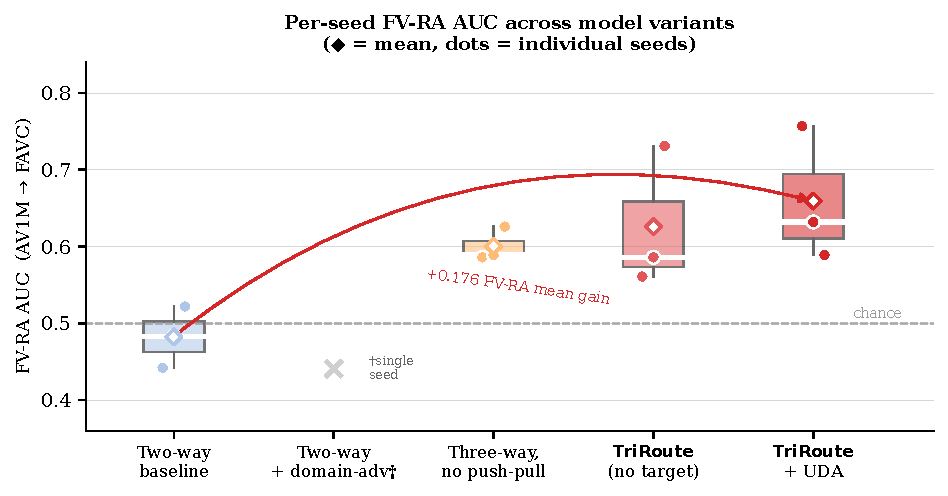
\includegraphics[width=0.72\linewidth]{seed_variance.pdf}
    \caption{Run-to-run FV-RA AUC for each model variant. Boxes show the interquartile range; the diamond marks the mean; individual dots show independent runs. The gain is consistent across runs and is not driven by a single outlier.}
    \label{fig:seed_variance}
\end{figure}

\paragraph{Reverse-direction generalisation (FAVC $\to$ AV1M).}
To verify that the routing benefit is not specific to the AV1M$\to$FAVC direction, we additionally train each ablation variant on FakeAVCeleb and evaluate on the AV-Deepfake1M validation split ($N=2{,}000$). Domain pseudo-labels in this direction are derived from a speaker-group hash within FAVC; the UDA variant additionally uses unlabelled real-only AV1M clips as target-domain identity. Table~\ref{tab:reverse} reports overall AUC/AP as mean$\,\pm\,$std over repeated runs. \method\ in the no-target-data setting again attains the best overall AUC ($0.747$), improving over the two-way baseline by $+0.077$ and over the three-way no-push-pull variant by $+0.064$. Unlike the AV1M$\to$FAVC direction, the UDA variant does not further improve the overall score on this much smaller and noisier target split; we attribute this to the limited diversity of FAVC-side training real audio for absorbing AV1M shortcut structure, and report the result without bolding to avoid overclaiming.

\begin{table}[t]
    \centering
    \caption{Reverse-direction cross-domain detection (FAVC $\to$ AV1M val, $N=2{,}000$). Each numeric cell reports overall AUC/AP, mean$\,\pm\,$std over repeated runs. All variants are trained on FakeAVCeleb; source-side nuisance labels come from a within-FAVC speaker-group hash; the UDA variant additionally uses unlabelled real-only AV-Deepfake1M clips as target-domain identity (no AV1M manipulation labels are used). The two-way DANN/CORAL controls from Table~\ref{tab:main} are omitted because they are not part of the reverse-direction sweep.}
    \label{tab:reverse}
    \small
    \begin{tabular}{llcc}
        \toprule
        Method & Structure & Overall AUC & Overall AP \\
        \midrule
        Two-way baseline                 & two-way factorization        & $0.670 \pm 0.032$ & $0.812 \pm 0.014$ \\
        Three-way, no domain push-pull   & three-way factorization      & $0.683 \pm 0.048$ & $0.822 \pm 0.033$ \\
        \method, no target data (ours)   & three-way + push-pull        & $\mathbf{0.747 \pm 0.078}$ & $\mathbf{0.864 \pm 0.052}$ \\
        \method\ + UDA (ours)            & three-way + push-pull + UDA  & $0.689 \pm 0.051$ & $0.813 \pm 0.017$ \\
        \bottomrule
    \end{tabular}
\end{table}

\subsection{Subspace Evidence: Stronger Routing, Not Full Invariance}

Table~\ref{tab:probe} summarizes representative probe results for the main visual subspaces. The most important pattern is that the visual-unique factor of \method\ is the strongest OOD carrier: its AV1M$\rightarrow$FAVC probe AUC reaches $0.924$, substantially above the two-way task branch ($0.705$) and above the shared visual factors in the three-way models. At the same time, all of these subspaces remain highly domain-predictive, with domain-probe AUCs above $0.96$. This is why we do not interpret the gain as evidence of full domain invariance. The safer and better-supported interpretation is that three-way factorization exposes a usable visual-unique channel and makes it easier for the final detector to route FV-RA decisions through that channel. Figure~\ref{fig:analysis} (left) displays these numbers visually alongside the corresponding domain-probe AUCs.

The intervention-based analysis tables below should be interpreted within their own protocols. Their baseline values are reported only to contextualize the intervention-induced change on the FV-RA subset, rather than to replace the headline benchmark numbers in Table~\ref{tab:main}.

\begin{table}[t]
    \centering
    \caption{Representative probe AUCs for key visual subspaces. The OOD probe is trained on AV1M and evaluated on the FAVC 70/30 test split; the domain probe measures dataset predictability. The visual-unique factor is the strongest OOD carrier, but it is not domain-invariant.}
    \label{tab:probe}
    \small
    \begin{tabular}{lccc}
        \toprule
        Subspace & Dim. & OOD probe & Domain probe \\
        \midrule
        Two-way task branch $Z_c$ & 1024 & $0.705$ & $0.998$ \\
        Two-way visual factor $v_c$ & 512 & $0.891$ & $0.994$ \\
        Three-way shared visual $s_v$ & 256 & $0.814$ & $0.992$ \\
        Three-way unique visual $u_v$ & 256 & $0.825$ & $0.967$ \\
        \method\ shared visual $s_v$ & 256 & $0.726$ & $0.989$ \\
        \method\ unique visual $u_v$ & 256 & $\mathbf{0.924}$ & $0.976$ \\
        \bottomrule
    \end{tabular}
\end{table}

\begin{table}[t]
    \centering
    \caption{Head-ablation analysis on FV-RA AUC. Each row zeros out one branch of the trained model and measures the FV-RA drop ($\Delta$FV-RA). Larger drop indicates heavier routing dependence on that branch. Baseline and ablated values should be compared within this intervention protocol rather than directly against Table~\ref{tab:main}. All rows report the mean over three independent seeds.}
    \label{tab:ablation}
    \resizebox{\linewidth}{!}{%
    \begin{tabular}{llccc}
        \toprule
        Model & Ablation & Baseline FV-RA & Ablated FV-RA & $\Delta$FV-RA \\
        \midrule
        Two-way baseline & mask visual task branch & $0.495$ & $0.461$ & $-0.034$ \\
        Three-way, no domain push-pull & mask visual branches & $0.586$ & $0.473$ & $-0.113$ \\
        \method & mask manipulation ($u_v$) & $0.721$ & $0.366$ & $\mathbf{-0.354}$ \\
        \bottomrule
    \end{tabular}}
\end{table}

\begin{figure}[t]
    \centering
    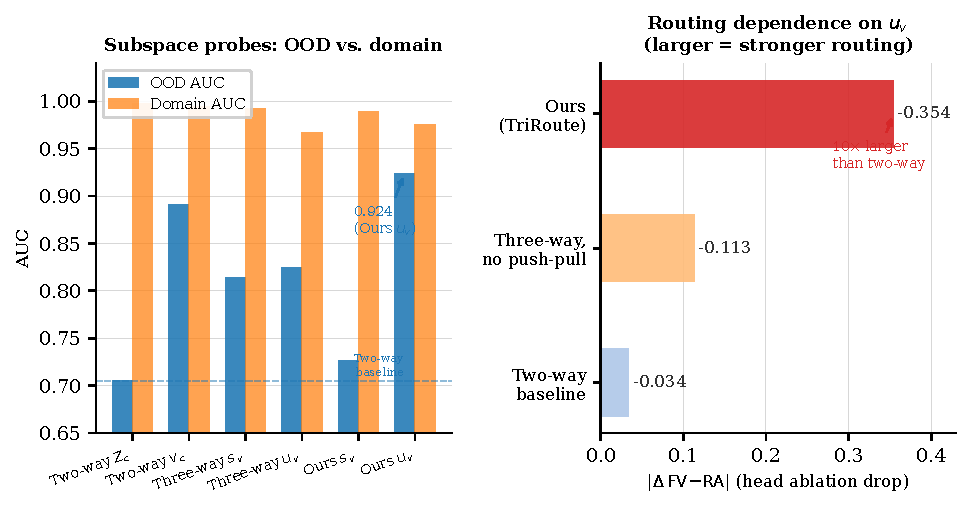
\includegraphics[width=0.97\linewidth]{analysis.pdf}
    \caption{\textbf{Left}: OOD probe AUC and domain-probe AUC for each visual subspace. The visual-unique channel of \method\ ($u_v$, rightmost pair) achieves the highest OOD AUC ($0.924$) while remaining strongly domain-predictive ($0.976$), supporting a routing rather than invariance explanation. \textbf{Right}: Head-ablation routing sensitivity ($|\Delta\text{FV-RA}|$ when the visual branch is masked). \method's FV-RA decision is $10\times$ more dependent on the visual-unique manipulation factor than the two-way baseline, demonstrating that factorization changes which evidence the detector uses.}
    \label{fig:analysis}
\end{figure}

\subsection{Routing Evidence: Head Ablation}

Table~\ref{tab:ablation} quantifies how strongly each model's FV-RA performance depends on its visual branches (also visualised in Figure~\ref{fig:analysis}, right). For the two-way baseline, zeroing the visual task branch causes a negligible drop of $-0.034$, confirming that the trained detector barely uses visual evidence for FV-RA decisions. For three-way factorization without domain push-pull, masking visual branches causes a larger drop ($-0.113$), indicating partial visual usage. For \method, masking the visual-unique manipulation factor alone causes a $-0.354$ drop, demonstrating that the FV-RA decision is routed primarily through this branch. The two-way model is just as routing-sensitive in the opposite direction: masking its audio branch drops in-domain AUC from 0.997 to 0.528, confirming audio dominance rather than visual capacity failure. This asymmetry is precisely what the three-way factorization is designed to break.

Figure~\ref{fig:routing} provides direct qualitative evidence for this routing pattern on held-out FakeAVCeleb clips. We select one correctly classified FV-RA fake clip and one correctly classified real clip from a representative \method\ checkpoint, then plot per-frame factor norms. The fake clip shows a sharp visual-unique excursion $\|u_v^t\|$ at the same time as an elevated residual response, while the real clip has a comparatively flat $\|u_v^t\|$ trace and a higher residual baseline. This pattern is consistent with the head-ablation finding that the FV-RA decision uses $u_v$ as the discriminative visual route, while $r_v$ carries nuisance/background variation rather than serving as the task path.

\begin{figure}[t]
    \centering
    
\includegraphics[width=0.97\linewidth]{routing_map.pdf}
    \caption{Per-frame routing activation from a real forward pass of a representative \method\ checkpoint on held-out FakeAVCeleb clips. \textbf{Top}: a correctly classified FV-RA fake clip, where the visual-unique factor ($u_v$, blue) shows a sharp transient response. \textbf{Bottom}: a correctly classified real clip, where $u_v$ remains comparatively flat. The residual factor ($r_v$, orange) remains elevated as a nuisance/background channel rather than being read by the task head.}
    \label{fig:routing}
\end{figure}

\subsection{Input-Level Routing Verification}

The head-ablation analysis zeroes out internal model components, which could conflate routing with capacity effects. As a complementary and model-agnostic test, we perturb the \emph{input features} on the FAVC FV-RA category and measure the resulting AUC change. This is a direct input-side intervention: if the trained head routes FV-RA decisions through the visual channel, full visual masking should cause a large drop; full audio masking, by contrast, should be neutral or beneficial (since FV-RA has real audio, masking it removes a potentially misleading signal).

Table~\ref{tab:perturbation} reports mean FV-RA AUC over repeated runs at full audio masking ($p=1.0$) and full visual masking ($p=1.0$). Two patterns stand out. First, the two-way baseline barely changes under either masking ($\Delta_{\mathrm{audio}}=-0.021$, $\Delta_{\mathrm{visual}}=-0.077$), consistent with a model near chance on FV-RA that is not strongly routing through either modality. Second, \method\ shows a strongly asymmetric profile: full audio masking \emph{improves} FV-RA ($+0.039$) while full visual masking causes a large drop ($-0.265$), a $3.4\times$ larger sensitivity to visual masking than the two-way baseline. The improvement under audio masking is consistent with visual routing: the model is actively suppressing a misleading real-audio signal when the routing is correctly established. Three-way factorization without push-pull shows an intermediate profile ($\Delta_{\mathrm{audio}}=+0.040$, $\Delta_{\mathrm{visual}}=-0.137$), matching the intermediate FV-RA AUC in Table~\ref{tab:main}.

\begin{table}[t]
    \centering
    \caption{FV-RA AUC under full input masking on the FakeAVCeleb FV-RA category. Each row reports the mean over repeated runs. $\Delta$ = masked AUC $-$ baseline AUC. A positive $\Delta_{\mathrm{audio}}$ indicates that removing the audio signal \emph{helps} FV-RA detection, i.e., the model is actively exploiting the visual channel and suppressing misleading real-audio signal. The \method\ row uses the UDA variant. Baseline values should be interpreted within this intervention protocol; the relative ordering matches the main table.}
    \label{tab:perturbation}
    \small
    \begin{tabular}{lcccc}
        \toprule
        Model & Baseline & $\Delta_{\mathrm{audio}}$ (full) & $\Delta_{\mathrm{visual}}$ (full) & Relative visual sensitivity \\
        \midrule
        Two-way baseline        & $0.546$ & $-0.021$ & $-0.077$ & $1.0\times$ \\
        Three-way, no push-pull & $0.616$ & $+0.040$ & $-0.137$ & $1.8\times$ \\
        \method\ (ours)         & $\mathbf{0.757}$ & $\mathbf{+0.039}$ & $\mathbf{-0.265}$ & $\mathbf{3.4\times}$ \\
        \bottomrule
    \end{tabular}
\end{table}

\subsection{Corrected Artifact Control}

A potential confound in AV1M-trained models is leading silence: fabricated clips sometimes begin with audio-free frames that are absent in authentic samples. We therefore evaluate a leading-silence-trimmed version that removes raw-waveform leading silence prior to AV-HuBERT feature extraction. Table~\ref{tab:silence_control} shows that FV-RA performance remains essentially stable across all models after trimming, while RV-FA and FV-FA drop substantially. This control therefore does not support the hypothesis that the visual-fake gain is driven by a leading-silence artifact; instead, the artifact mainly inflates audio-fake categories.

\begin{table}[t]
    \centering
    \caption{Leading-silence artifact control. Values are per-category AUC before and after true trimming of leading silence, with $\Delta$ = trimmed $-$ untrimmed. FV-RA remains stable across all models, indicating that the visual-routing gain is not explained by leading-silence artifacts.}
    \label{tab:silence_control}
    \small
    \begin{tabular}{llcccc}
        \toprule
        Model & Condition & Overall & RV-FA & FV-RA & FV-FA \\
        \midrule
        Two-way baseline & Untrimmed & $0.7772$ & $1.0000$ & $0.5119$ & $0.9995$ \\
        Two-way baseline & Trimmed   & $0.7011$ & $0.9625$ & $0.5079$ & $0.8584$ \\
        Two-way baseline & $\Delta$  & $-0.0761$ & $-0.0375$ & $\mathbf{-0.0040}$ & $-0.1411$ \\
        \midrule
        Three-way, no push-pull & Untrimmed & $0.8309$ & $0.9985$ & $0.6340$ & $0.9957$ \\
        Three-way, no push-pull & Trimmed   & $0.7808$ & $0.9492$ & $0.6259$ & $0.9089$ \\
        Three-way, no push-pull & $\Delta$  & $-0.0501$ & $-0.0493$ & $\mathbf{-0.0081}$ & $-0.0868$ \\
        \midrule
        \method, no target data & Untrimmed & $0.8410$ & $1.0000$ & $0.6543$ & $0.9973$ \\
        \method, no target data & Trimmed   & $0.7538$ & $0.9034$ & $0.6544$ & $0.8341$ \\
        \method, no target data & $\Delta$  & $-0.0872$ & $-0.0966$ & $\mathbf{+0.0001}$ & $-0.1632$ \\
        \bottomrule
    \end{tabular}
\end{table}

\subsection{Domain Label Quality}
\label{sec:domain_label_quality}

A natural question is how much the quality of nuisance supervision matters. The speaker-group pseudo-label is not a target-domain label: it partitions source clips by speaker identity and is therefore closer to a weak speaker-group nuisance proxy than to true knowledge of the AV1M-to-FAVC domain gap. It does not directly encode codec differences, acquisition conditions, or any FAVC-specific artifact. Yet this coarse signal already yields a $+0.208$ FV-RA gain over the two-way baseline ($0.523 \to 0.731$). Providing a more accurate source-target contrast via the UDA setting (unlabelled FAVC real-only clips) yields a further gain ($0.731 \to 0.804$, $+0.073$). We therefore interpret nuisance supervision as helpful but secondary to the representation split itself.

\subsection{Comparison in AVH-Align Protocol}

Table~\ref{tab:avhalign_comparison} replicates the structure of Table~2 in \citet{smeu2025avhalign}, reporting AUC and AP on the FakeAVCeleb 70/30 test split and AV-Deepfake1M validation set ($N=2{,}000$), with and without leading-silence trimming. Baseline rows are reproduced from \citet{smeu2025avhalign}. Our rows report the source-side nuisance-label (no-target-data) variant. This table complements Table~\ref{tab:external_category}: Table~\ref{tab:external_category} isolates the FV-RA visual-routing failure mode, while this table gives broader aggregate context against published audio-visual baselines.

We treat this comparison as supportive rather than central because it mixes source-supervised AV1M training with unsupervised speech-pretraining regimes. The most direct comparison is the supervised AV1M-trained AVH-Align row, since it uses the same transfer direction and compatible AV-HuBERT features. Under that comparison, after leading-silence trimming, \method\ remains clearly stronger on FAVC ($84.3$ vs.\ $70.8$ AUC). The unsupervised VoxCeleb2-pretrained rows are included for context rather than as matched baselines; their higher FAVC numbers indicate the remaining benefit of broader speech pretraining rather than a failure of the routing analysis.
Note that \method\ trained directly on FAVC reaches near-ceiling in-domain performance (AUC $99.6$, lower block of Table~\ref{tab:avhalign_comparison}), indicating that the AV1M$\rightarrow$FAVC gap is not a model-capacity limitation of \method\ but a manifestation of cross-dataset shift.

\begin{table}[t]
    \centering
    \caption{Comparison with \citet{smeu2025avhalign} Table~2 baselines on FakeAVCeleb (FAVC) 70/30 test split and AV-Deepfake1M (AV1M) validation set. Values are percentages. Trim:$\checkmark$ denotes leading-silence-trimmed evaluation. Baseline rows are reproduced from \citet{smeu2025avhalign}; our rows report the source-side nuisance-label (no-target-data) variant averaged over repeated runs. Bold highlights the best source-supervised AV1M-trained result within our matched comparison block, not the unsupervised VoxCeleb2-pretrained rows. FAVC-trained rows additionally show the reverse-direction transfer; FAVC Trim:$\checkmark$ columns are identical to Trim:$\times$ for FAVC-trained models because leading-silence trimming targets AV1M-synthesized clips.}
    \label{tab:avhalign_comparison}
    \resizebox{\linewidth}{!}{%
    \begin{tabular}{llllcccccccc}
        \toprule
        & & & & \multicolumn{4}{c}{Metric: AUC} & \multicolumn{4}{c}{Metric: AP} \\
        \cmidrule(lr){5-8}\cmidrule(lr){9-12}
        & & & & \multicolumn{2}{c}{FakeAVCeleb} & \multicolumn{2}{c}{AV-Deepfake1M} & \multicolumn{2}{c}{FakeAVCeleb} & \multicolumn{2}{c}{AV-Deepfake1M} \\
        \cmidrule(lr){5-6}\cmidrule(lr){7-8}\cmidrule(lr){9-10}\cmidrule(lr){11-12}
        Method & Mod. & Train type & Train data & Trim:$\times$ & Trim:$\checkmark$ & Trim:$\times$ & Trim:$\checkmark$ & Trim:$\times$ & Trim:$\checkmark$ & Trim:$\times$ & Trim:$\checkmark$ \\
        \midrule
        AVH-Align/sup \citep{smeu2025avhalign} & AV & sup. & FAVC & 99.2 & 99.2 & 69.0 & 63.6 & 100.0 & 100.0 & 84.1 & 82.2 \\
        AVH-Align/sup \citep{smeu2025avhalign} & AV & sup. & AV1M & 77.5 & 70.8 & 100.0 & 83.1 & 99.4 & 99.1 & 100.0 & 94.4 \\
        AVAD \citep{feng2023avad}               & AV & unsup. & LRS       & 84.5 & 84.7 & 54.3  & 54.3 & 99.5  & 99.5  & 76.3  & 76.3 \\
        SpeechForensics \citep{liang2024speechforensics} & AV & unsup. & VoxCeleb2 & 98.8 & 98.8 & 68.8 & 68.2 & 100.0 & 100.0 & 83.7 & 83.5 \\
        AVH-Align \citep{smeu2025avhalign}      & AV & unsup. & VoxCeleb2 & 94.6 & 94.6 & 85.9  & 83.5 & 99.8  & 99.8  & 94.3  & 93.5 \\
        \midrule
        Two-way baseline (ours)          & AV & sup. & AV1M & 77.9 & 69.7 & 99.8 & 74.7 & 99.4 & 99.0 & 99.9 & 90.1 \\
        Three-way, no push-pull (ours)   & AV & sup. & AV1M & 82.7 & 78.0 & 99.9 & 84.6 & 99.6 & 99.4 & 100.0 & 94.7 \\
        \method\ (ours)                  & AV & sup. & AV1M & \textbf{87.4} & \textbf{84.3} & \textbf{99.9} & \textbf{87.3} & \textbf{99.7} & \textbf{99.5} & \textbf{100.0} & \textbf{95.5} \\
        \midrule
        Two-way baseline (ours)          & AV & sup. & FAVC & 99.5 & 99.5 & 67.0 & 63.4 & 100.0 & 100.0 & 81.2 & 79.8 \\
        Three-way, no push-pull (ours)   & AV & sup. & FAVC & 99.7 & 99.7 & 68.3 & 65.1 & 100.0 & 100.0 & 82.2 & 80.4 \\
        \method\ (ours)                  & AV & sup. & FAVC & 99.6 & 99.6 & \textbf{74.7} & \textbf{67.7} & 100.0 & 100.0 & \textbf{86.4} & \textbf{82.2} \\
        \bottomrule
    \end{tabular}}
\end{table}

\subsection{Training Dynamics}

Figure~\ref{fig:training_dynamics} tracks the FV-RA AUC on held-out FAVC and the domain-probe AUC on $Z_{\mathrm{task}}$ over training epochs for \method. As the domain push-pull objective expels shortcut information from the task branch (falling domain-probe AUC on $Z_{\mathrm{task}}$), FV-RA AUC rises correspondingly. The residual branch simultaneously absorbs the expelled domain signal (rising domain-probe AUC on $Z_{\mathrm{res}}$). The two-way baseline FV-RA curve stays near chance throughout, confirming that the improvement is attributable to the factorized routing structure rather than extended training.

\begin{figure}[t]
    \centering
    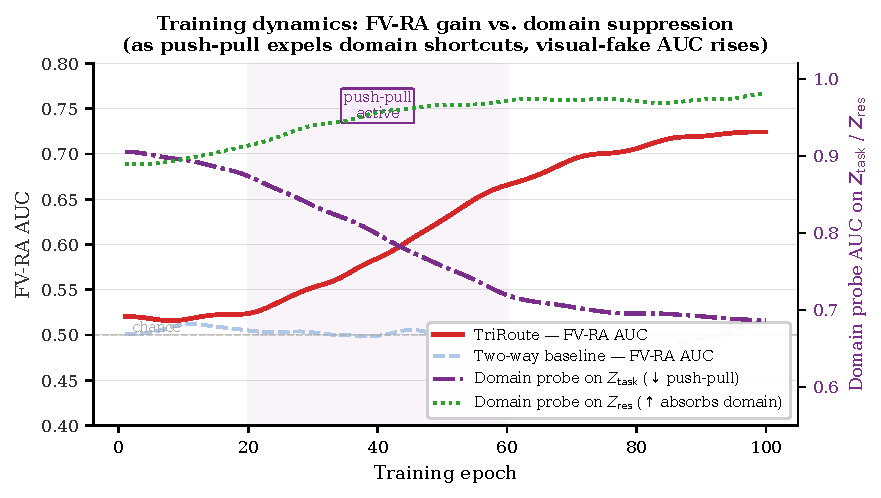
\includegraphics[width=0.82\linewidth]{training_dynamics.pdf}
    \caption{Training dynamics for \method. As domain push-pull suppresses shortcuts in $Z_{\mathrm{task}}$ (purple dash-dot, right axis), FV-RA AUC rises (red, left axis). The residual branch $Z_{\mathrm{res}}$ absorbs the expelled domain information (green dotted, right axis). The two-way baseline FV-RA stays near chance (blue dashed), isolating the factorization as the enabling condition.}
    \label{fig:training_dynamics}
\end{figure}

\subsection{Factor Geometry}

Figure~\ref{fig:tsne} visualises t-SNE embeddings of the two key factors from \method. The residual factor $Z_{\mathrm{res}}$ forms tight, dataset-separated clusters, confirming that it absorbs domain-specific nuisance. The task factor $Z_{\mathrm{task}}$ separates real from fake samples across all source domains without residual domain clustering, indicating that domain push-pull successfully discourages the shortcut from entering the prediction head.

\subsection{Supplementary External Support on AVLips}

To test whether the same ordering appears on a second external benchmark, we evaluated all three model families on AVLips and report mean results over repeated runs in Table~\ref{tab:avlips}. AVLips provides only binary real/fake labels without modality-category annotations (RV-FA, FV-RA, FV-FA), so only full-set AUC can be reported. The same ordering is preserved: the two-way baseline reaches $0.568$, three-way factorization without domain push-pull reaches $0.595$, and \method\ reaches $0.734$. This result is directionally consistent with the FakeAVCeleb benchmark and suggests that the routing-based improvement is not isolated to a single target dataset. We nevertheless treat AVLips as supportive rather than central evidence, because the run-to-run variance for \method\ is larger there than on FakeAVCeleb.

\begin{figure}[t]
    \centering
    
\includegraphics[width=0.97\linewidth]{tsne.pdf}
    \caption{t-SNE embeddings of the two key factors from a representative \method\ checkpoint. \textbf{Left}: the residual factor $Z_{\mathrm{res}}$ forms tight, dataset-specific clusters (colors), confirming it absorbs domain nuisance. \textbf{Right}: the task factor $Z_{\mathrm{task}}$ separates real (blue circles) from fake (red crosses) across all source domains, with no residual domain clustering, indicating that domain push-pull successfully discourages shortcut routing into the prediction head.}
    \label{fig:tsne}
\end{figure}

\begin{table}[t]
    \centering
    \caption{AVLips cross-dataset AUC averaged over independent runs. AVLips provides only binary real/fake labels, so per-modality-category breakdown is not available. Reported as supplementary directional evidence.}
    \label{tab:avlips}
    \small
    \begin{tabular}{lc}
        \toprule
        Method & Full AUC on AVLips \\
        \midrule
        Two-way baseline &  $0.5677$ \\
        Three-way, no domain push-pull &  $0.5954$ \\
        \method\ (ours) & $\mathbf{0.7340}$ \\
        \bottomrule
    \end{tabular}
\end{table}

\section{Limitations and Broader Impact}

\paragraph{Limitations.}
\method\ is still anchored to speech-related evidence, so it may be less effective on deepfakes with minimal speaking motion or on clips where the audio track is absent, replaced, or intentionally desynchronized for benign reasons. The main category-level gain is also concentrated in FV-RA, because RV-FA and FV-FA are already near ceiling in the AV1M$\rightarrow$FAVC protocol; this makes FV-RA the most diagnostic setting for visual routing, but it also limits how broadly the category-level result can be interpreted. The external supervised comparison is currently limited by the scarcity of published methods trained on AV1M and evaluated on FAVC under matched category annotations. Retraining additional baselines such as AVAD, SpeechForensics, and AVFF under the same AV1M$\rightarrow$FAVC protocol would strengthen the empirical comparison.

More specifically, our baseline block should be read as a mechanism-oriented comparison rather than an exhaustive leaderboard. We compare against the closest published compatible supervised bridge (AVH-Align/sup) and against internal controls designed to isolate routing effects, but we do not retrain a broader external baseline suite under the exact AV1M$\rightarrow$FAVC category protocol. Likewise, while DANN and CORAL provide two complementary global-alignment controls, we report them under matched default settings rather than a full GRL hyperparameter sweep; a stronger baseline audit would include a broader $\alpha$ sensitivity study and possibly alternative adversarial schedules.

The factorization introduces additional optimization complexity and benefits from some nuisance partition or domain contrast during training. As shown in Section~\ref{sec:domain_label_quality}, the speaker-group pseudo-label is an extremely weak proxy for the true domain gap, yet the factorization improves FV-RA substantially. The UDA setting provides an additional gain ($+0.073$) by supplying more accurate domain contrast via unlabelled target-domain real clips. Whether stronger or multi-source domain contrast could yield further gains remains an open question. Benchmark breadth is also still limited: FakeAVCeleb is the only fully analyzed target with category-level routing diagnostics, while AVLips is supplementary and the reverse-direction sweep shows higher variance. Finally, our routing evidence is mechanistic but not a formal causal proof: probes, branch ablations, input masking, and training dynamics all point to heavier use of the visual-unique factor, but future falsification tests should vary the capacity of $u_v$ and the residual branch directly.

\paragraph{Broader impact.}
Cross-domain deepfake detection can support content authentication, media forensics, and platform integrity. At the same time, any detector can be misused for surveillance or overconfident moderation, especially if its uncertainty is not surfaced. We therefore recommend reporting calibration, failure modes, and domain-shift sensitivity, and releasing models with clear usage restrictions and dataset documentation.

\section{Conclusion}

We proposed \method, a factorized audio-visual deepfake detector that separates shared content, modality-unique manipulation evidence, and residual domain-sensitive signal so that the prediction head is discouraged from solving the task through shortcut-heavy branches. Across the AV1M$\rightarrow$FAVC cross-domain benchmark, the main result is a substantial improvement on FV-RA, the diagnostic category that forces the detector to rely on visual manipulation evidence: global DANN and CORAL controls on a coarser two-way representation remain near chance ($0.478/0.952$ and $0.491/0.947$), while \method\ with source-side nuisance labels improves FV-RA to $0.731$ AUC and with UDA further to $0.804$ AUC. The gap between the two settings ($+0.073$) indicates that target-domain contrast can further strengthen the factorized routing mechanism. Subspace probes identify the visual-unique channel as the strongest OOD carrier, while head ablation and input-level perturbation both indicate heavier routing dependence on that channel. Together, these analyses support a routing-based interpretation of the cross-domain gain rather than a claim of full domain invariance. For cross-domain forensics, the central question is therefore less how to make every feature domain-invariant, and more how to structurally prevent the detector from using shortcut features it can otherwise see.
On FV-RA specifically, \method\ moves the closest AV1M-supervised external baseline (AVH-Align/sup, $0.519$ AUC) to $0.804$ AUC with UDA, a relative improvement of about $55\%$, shifting performance from near-chance transfer to a practically usable cross-domain detector on the visual-routing stress category.
We therefore view the present evidence as strongest for the routing mechanism itself under a deliberately diagnostic cross-domain setting, rather than as a final statement about universal superiority across datasets, baselines, or adaptation schedules.

\bibliographystyle{plainnat}
\bibliography{references}

\newpage
\input{checklist}

\end{document}
